% The practice exam (one sample, Div 2026-10-06): questions and solutions in one
% source. \input by midterm1-practice.tex (\solutionsfalse) and
% midterm1-practice-solutions.tex (\solutionstrue). Same format as the real
% exam, as the study guide describes it: three parts weighted equally at 10
% points each, each on its own sheet printed front and back, with name and
% CWID boxes on every sheet.
%   Part 1, ten multiple-choice questions in lecture order: two on lecture 4
%     (sunk cost, comparative advantage), two on lecture 6 (returns to scale,
%     average cost), one on lecture 7 (an elasticity from two points), and
%     one on lecture 12 (natural monopoly); lectures 8 to 12 are otherwise
%     tested in Parts 2 and 3 (Div, 2026-10-06).
%   Part 2, short-answer problems: four at 2.5 points, two explain and two
%     small problems with no lettered parts (Div, 2026-10-06). The explain
%     questions: the owned factory and student discounts (price
%     discrimination). The problems, each with a real-world lesson (Div):
%     markups on economy and luxury cars from their elasticities (lecture
%     12's car data, market power) and cross-price elasticities of SUVs and
%     electric cars with the price of gas (lecture 8).
%   Part 3, one long-form question, Lakeside Smoothies (Div, 2026-10-06): it
%     opens with the demand curve plotted with MR and MC and the $4 cost per
%     smoothie; (a) checks the plot's MR = MC at 50 by computing the 51st
%     smoothie's MR step by step, (b) Q* and P* with E and the price line
%     drawn, (c) CS, PS, and DWL shaded on the same page; on the back, (d)
%     and (e) CS and PS computed and explained, (f) to (h) the DWL buyers, a
%     Pareto-improving price, and DWL computed. No fixed cost and no extra
%     credit (Div cut both as redundant). Writing space is sized to each
%     answer.
% Reworked on 2026-10-06 (Div: match the structure on the study guide and
% follow it); Part 2 had been one long problem (the island ferry). This repo
% is public: keep notes about the real exam out of this file.
% Numbers are checked in figures/make_midterm1.py.

\ifsolutions
\docheader{Practice Exam: Solutions}{ECON 201}
\else
\sheet{Sheet 1 of 3}
\docheader{Practice Exam}{ECON 201}
\begin{notepanel}{Instructions}
\begin{itemize}
\item 65 minutes. Three parts, weighted equally at 10 points each, each on its own sheet printed front and back: Part 1, ten multiple-choice questions; Part 2, short-answer problems; Part 3, one long-form question.
\item Closed book and closed notes. A basic calculator is allowed. You will be given the help sheet separately.
\item Write your name and CWID, one digit per box, at the top of every sheet: the sheets are graded separately and matched by CWID.
\item Show your work in Parts 2 and 3.
\end{itemize}
\end{notepanel}
\fi

\section{Part 1: Multiple Choice \pts{10}}
\where{1 point each. Fill the bubble of the one best answer.}

\begin{enumerate}\setlength{\itemsep}{4pt}

\mcq{Kai runs a food truck. After paying for food, fuel, and the permit, the books show a profit of \$40,000 a year. Kai could instead earn \$55,000 a year as a chef at a restaurant. Kai's economic rent from running the truck is}
  {\$40,000, the profit on the books.}
  {$-\$15{,}000$: an economic loss.}
  {\$95,000.}
  {\$15,000.}
\sol{(B). Economic rent is net benefit minus opportunity cost: $40{,}000 - 55{,}000 = -15{,}000$. The books leave out the chef's salary Kai gives up.}

\mcq{A studio has spent \$2 million on a video game that is half finished, and it cannot get that money back. Finishing the game would cost \$1 million more, and the finished game would bring in \$1.5 million. The studio should}
  {stop, since its total cost of \$3 million is more than \$1.5 million.}
  {stop, since it has already lost \$2 million.}
  {finish it only if it brings in at least \$3 million.}
  {finish it, since \$1.5 million is more than the \$1 million it still costs.}
\sol{(D). The \$2 million is a sunk cost: it is spent whichever choice the studio makes, so it should not affect the decision. Finishing adds \$1.5 million for \$1 million more.}

\mcq{In an hour, Ana can bake 6 loaves or 12 muffins, and Raj can bake 2 loaves or 8 muffins. Who has the comparative advantage in muffins?}
  {Ana, since she bakes more muffins.}
  {Raj, since a muffin costs him $\tfrac{1}{4}$ loaf and costs Ana $\tfrac{1}{2}$ loaf.}
  {Neither, since Ana has the absolute advantage in both goods.}
  {Ana, since a muffin costs her 2 loaves.}
\sol{(B). A muffin costs Ana $6/12 = \tfrac{1}{2}$ loaf and Raj $2/8 = \tfrac{1}{4}$ loaf, so Raj gives up less to make one. Ana is better at making both, but she cannot have the comparative advantage in both.}

\mcq{A bakery's customers believe they cannot find its sourdough anywhere else. Compared with a bakery whose bread is the same as its rivals', it}
  {can raise its price and keep many of its buyers.}
  {must charge the same price as its rivals.}
  {faces no trade-off between price and quantity.}
  {loses all its buyers if it raises its price.}
\sol{(A). A differentiated product has features buyers value and believe they cannot find elsewhere, so a higher price loses some buyers but not all. The trade-off remains: by the law of demand, a higher price still sells less.}

\mcq{A furniture maker doubles all of its inputs: workers, machines, materials, and space. Its output less than doubles. The firm has}
  {increasing returns to scale.}
  {constant returns to scale.}
  {decreasing returns to scale, or diseconomies of scale.}
  {economies of scale.}
\sol{(C). Output that less than doubles when every input doubles is decreasing returns to scale, also called diseconomies of scale.}

\mcq{A print shop pays \$600 a month for its space, and each poster costs it \$2 in paper and ink. What is its average cost per poster if it prints 100 posters a month, and if it prints 300?}
  {\$8 and \$4.}
  {\$2 and \$2.}
  {\$6 and \$2.}
  {\$8 and \$8.}
\sol{(A). $C(Q) = 600 + 2Q$, so $\text{AC} = C(Q)/Q$: $(600 + 200)/100 = 8$ and $(600 + 600)/300 = 4$. Equivalently $\text{AC} = 2 + 600/Q$: it falls toward the \$2 MC as the fixed cost is spread over more posters. Choice (C) leaves out the \$2 per poster.}

\mcq{A bus company raises its fare from \$2.00 to \$2.20, and daily riders fall from 10,000 to 9,500. The price elasticity of demand is}
  {2, so demand is elastic.}
  {0.5, so demand is elastic.}
  {0.5, so demand is inelastic.}
  {5, so demand is elastic.}
\sol{(C). The fare rises $\tfrac{2.20 - 2.00}{2.00} \times 100 = 10\%$ and riders fall $\tfrac{9{,}500 - 10{,}000}{10{,}000} \times 100 = -5\%$, so $\varepsilon = -\tfrac{-5\%}{10\%} = 0.5$. Below 1, so demand is inelastic.}

\mcq{A store sells headphones for \$120 a pair to everyone, and each pair costs it \$40. A buyer who values a pair at \$70 does not buy. Selling that buyer one pair at \$60, while everyone else still pays \$120, would}
  {make the store worse off, since \$60 is below \$120.}
  {make the other buyers worse off.}
  {add to the deadweight loss.}
  {be a Pareto improvement: the buyer gains \$10, the store \$20, and nobody loses.}
\sol{(D). The buyer gains $70 - 60 = 10$ and the store $60 - 40 = 20$, and no one else's price changes. A sale to a buyer whose WTP is above MC is the surplus that a single price leaves out, the deadweight loss.}

\mcq{Which of these is most likely to be a natural monopoly?}
  {Restaurants in a large city.}
  {The water pipes that serve a town.}
  {A drug company that holds the patent on a new medicine.}
  {Wheat farms.}
\sol{(B). A market is a natural monopoly when one firm can supply all of it at a lower average cost than two or more firms could. Laying the pipes is a huge fixed cost and serving one more home costs little, so one network serves the whole town more cheaply than two would. The drug company is a monopoly too, but its market power comes from the patent, not from its costs: when the patent expires, makers of generics enter. Restaurants and wheat farms have many sellers.}

\mcq{Two gas stations face each other across a road. Their prices are likely to be lowest when}
  {most drivers compare prices and fill up at the cheaper station.}
  {most drivers are loyal to one station and fill up there at any price.}
  {drivers see the two stations' gas as different.}
  {both stations have low fixed costs.}
\sol{(A). When drivers compare prices, each station can win many of them by undercutting the other, so competition pushes both prices down. Loyal customers and differentiation make demand less elastic and prices higher; a fixed cost does not change the best price.}

\end{enumerate}

\ifsolutions\clearpage\else\sheet{Sheet 2 of 3. Show your work.}\fi
\section{Part 2: Short-Answer Problems \pts{10}}
\where{Four questions, 2.5 points each. Answer 1 and 2 in two or three sentences, using the ideas from class; show your work in 3 and 4.}

\sa{1}{2.5} The owners of a firm bought their factory outright years ago. A new manager argues that since it is paid for, using it costs nothing. What is missing from that argument?
\ifsolutions\else\vfill\fi
\sol{The money tied up in the factory could be earning a return if invested elsewhere, or the factory could be sold or rented out (1 pt). That forgone return, the opportunity cost of capital, is a real cost of using the factory even though no bill arrives for it (1 pt), and to keep its investors the firm has to earn at least that much (0.5 pt).}

\sa{2}{2.5} Cinemas, museums, and software companies routinely charge students less than other customers for exactly the same thing. What is this called, and why do firms do it?
\ifsolutions\else\vfill\fi
\sol{Price discrimination: charging different buyers different prices based on their willingness to pay (1 pt). Students typically have a lower willingness to pay. At the regular price many of them would not buy, even though they value the product above what it costs the firm to serve them. A student price brings them in, while everyone else still pays the regular price. Each extra sale brings in more than it costs, so the firm's profit rises; and those sales create surplus that was lost before, so the deadweight loss shrinks (1.5 pts).}

\ifsolutions\else\clearpage\fi
\sa{3}{2.5} Economists estimate that, at their profit-maximizing prices, the price elasticity of demand is about 6 for a small economy car and about 3 for a luxury car. Use the markup rule to find each car's markup. What does a markup measure, and why is the luxury car's higher?
\ifsolutions\else\vfill\fi
\sol{The markup rule, $(P - \text{MC})/P = 1/\varepsilon$, gives $1/6 \approx 17\%$ for the economy car and $1/3 \approx 33\%$ for the luxury car (1 pt). The markup is the share of the price above marginal cost, how far a firm can price above its cost: a measure of its market power (0.5 pt). An economy car has many close substitutes, so a small price rise sends buyers to other models: demand is elastic and the markup low. A luxury car has fewer close substitutes, so its demand is less elastic: the maker has more market power and sets a higher markup (1 pt).}

\sa{4}{2.5} Suppose the price of gasoline rises 25\%. Sales of large SUVs fall 10\%, and sales of electric cars rise 15\%. Find the cross-price elasticity of demand for each with respect to the price of gas, and say what each number tells you about the pair.
\ifsolutions\else\vfill\fi
\sol{SUVs: $-10\%/25\% = -0.4$. Negative, so SUVs and gas are complements: higher gas prices make a car that burns a lot of gas less attractive (1.25 pts). Electric cars: $15\%/25\% = 0.6$. Positive, so they are substitutes for gas: higher gas prices send buyers toward cars that do not use gas (1.25 pts).}

\ifsolutions\clearpage\else\sheet{Sheet 3 of 3. Show your work.}\fi
\section{Part 3: Long-Form Question \pts{10}}

\subsection{Lakeside Smoothies}

Lakeside Smoothies is a stand at a lake. Its demand curve is
\[ Q = 120 - 5P, \qquad\text{or equivalently}\qquad P = 24 - \frac{Q}{5}, \]
where $P$ is the price of a smoothie and $Q$ is smoothies sold per day. Each smoothie costs the stand \$4 in fruit, ice, and labor. The graph plots the demand curve with the stand's marginal revenue (MR) and marginal cost (MC).

\begin{center}
\ifsolutions
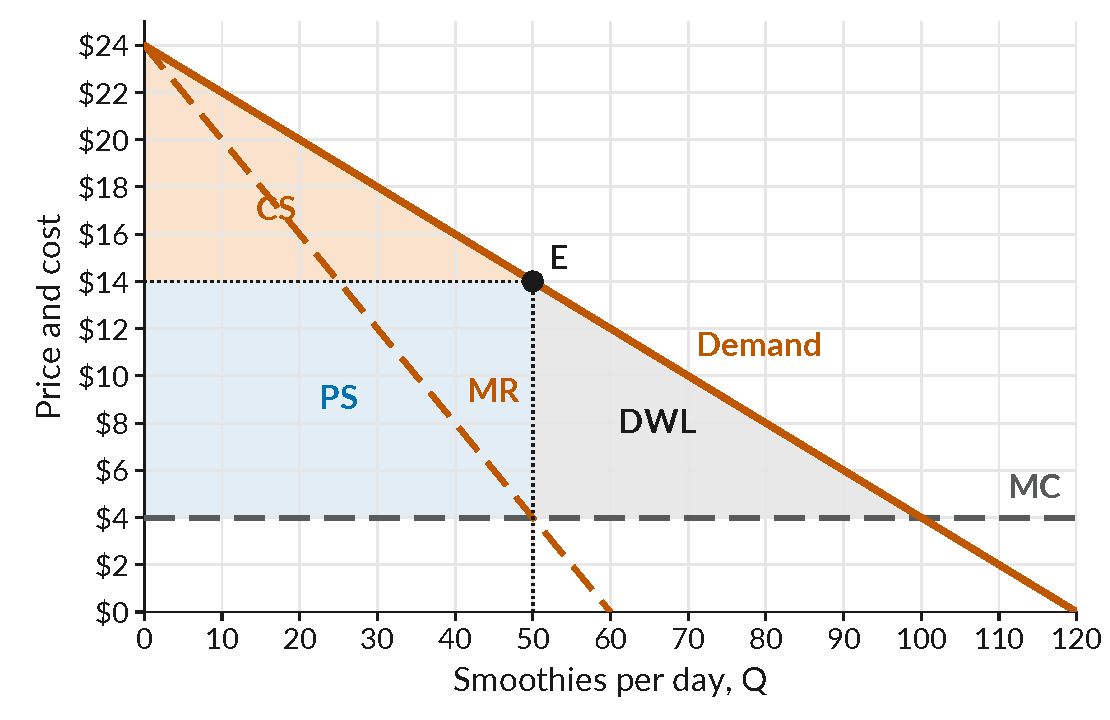
\includegraphics[width=0.72\linewidth, alt={Price and cost from 0 to 24 dollars on the vertical axis, smoothies per day from 0 to 120 on the horizontal, gridlines every 2 dollars and every 10 smoothies. Demand falls in a straight line from 24 dollars at zero to zero at 120. A dashed marginal revenue line falls twice as steeply from the same point, reaching zero at 60. Marginal cost is a flat dashed line at 4 dollars. A dotted price line at 14 dollars meets the demand curve at the point E, at 50 smoothies. Consumer surplus is shaded above 14 dollars out to 50, producer surplus between 4 and 14 dollars out to 50, and deadweight loss between marginal cost and demand from 50 to 100.}]{figures/smoothies-key.pdf}
\else
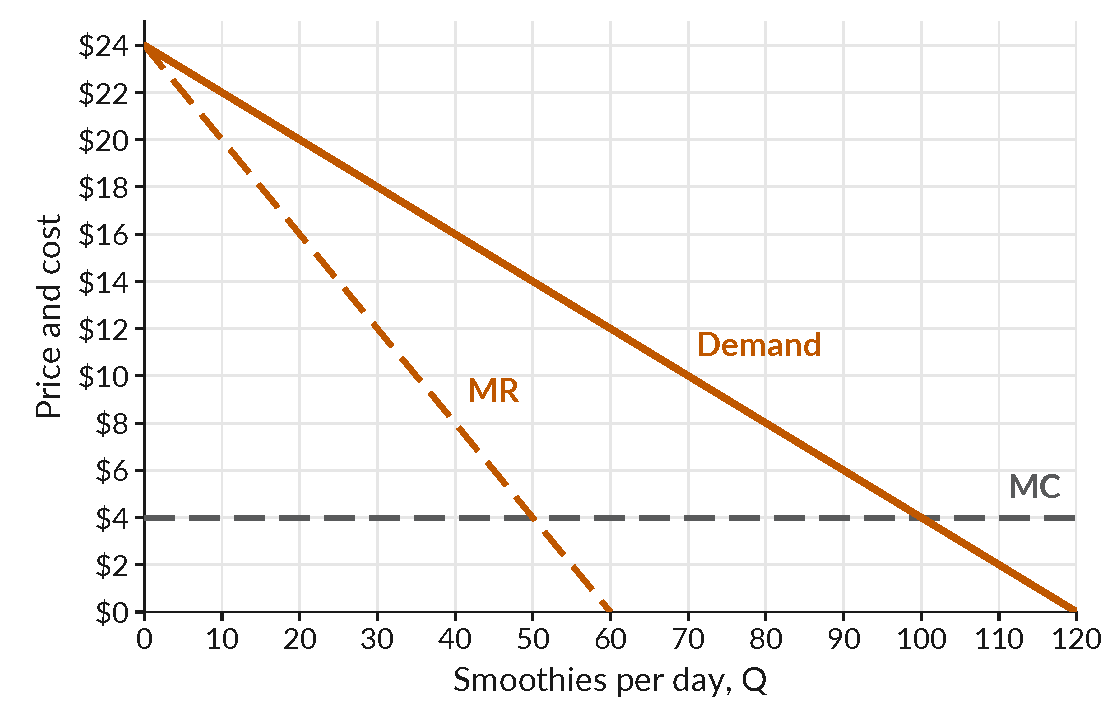
\includegraphics[width=0.72\linewidth, alt={A plotting grid, price and cost from 0 to 24 dollars on the vertical axis with gridlines every 2 dollars, and smoothies per day from 0 to 120 on the horizontal axis with gridlines every 10. Demand falls in a straight line from 24 dollars at zero to zero at 120. A dashed marginal revenue line falls twice as steeply from the same point, reaching zero at 60. Marginal cost is a flat dashed line at 4 dollars. Nothing is marked.}]{figures/smoothies.pdf}
\fi
\end{center}

\qpart{a}{2} On the plot, MR at 50 smoothies is exactly \$4, equal to MC. Check this for the 51st smoothie. Find the price that sells 51 smoothies, calculate revenue at 51 and at 50 smoothies, and take $\text{MR} = R(51) - R(50)$. What does your answer tell the stand about selling the 51st smoothie?
\work{5}
\sol{To sell 51 the price must be $P = 24 - 51/5 = 13.80$, so $R(51) = 13.80 \times 51 = 703.80$, while $R(50) = 14 \times 50 = 700$ (1 pt). $\text{MR} = 703.80 - 700 = 3.80$ (0.5 pt), just below \$4, as the plot shows. The 51st smoothie adds \$3.80 to revenue but \$4 to cost, so selling it lowers profit by 20 cents: the stand should stop at 50, where MR meets MC (0.5 pt).}

\qpart{b}{1.5} What are the profit-maximizing quantity and price? Mark that point, $E$, on the demand curve in the graph above, and draw the price line through it.
\work{1.5}
\sol{50 smoothies, where MR meets MC (0.5 pt). The price that sells 50 is \$14, on the demand curve straight above (0.5 pt), so $E$ is at $(50, 14)$, with the price line at \$14 (0.5 pt).}

\qpart{c}{1.5} On the graph, shade and label the consumer surplus, the producer surplus, and the deadweight loss.
\work{0.5}
\sol{See the plot above, where all three are shaded.}

\ifsolutions\else\clearpage\fi
For the rest of the problem, use the areas you shaded on the front of this sheet.

\qpart{d}{1.5} Compute the consumer surplus, and explain why that area measures what buyers gain.
\ifsolutions\else\vspace{\stretch{5}}\fi
\sol{$\text{CS} = \tfrac{1}{2} \times 50 \times (24 - 14) = \$250$ (0.5 pt). Each buyer gains the difference between what a smoothie is worth to them, the height of the demand curve at their place in line, and the \$14 they pay; adding those gains over the 50 buyers fills the area between the demand curve and the price line (1 pt).}

\qpart{e}{1.5} Compute the producer surplus, and explain why that area measures what the stand gains.
\ifsolutions\else\vspace{\stretch{5}}\fi
\sol{$\text{PS} = (14 - 4) \times 50 = \$500$ (0.5 pt). On each smoothie the stand gains the price minus the cost of that smoothie, $14 - 4 = \$10$, the same on every one, so the gains add up to a rectangle 10 high and 50 wide (1 pt).}

\qpart{f}{0.5} Which buyers value a smoothie above its \$4 cost but do not buy at \$14? Give the range, from the \rule{1.2em}{0.4pt}th to the \rule{1.2em}{0.4pt}th buyer.
\ifsolutions\else\vspace{\stretch{2}}\fi
\sol{From the graph we can see that the demand curve lies below the \$14 price and above the \$4 MC between 50 and 100 smoothies, so these are the 51st to the 99th buyers.}

\qpart{g}{0.5} Give a price at which selling a smoothie to the 75th buyer would be a Pareto improvement.
\ifsolutions\else\vspace{\stretch{2}}\fi
\sol{The 75th buyer's WTP is $24 - 75/5 = \$9$, above the \$4 cost, so any price between \$4 and \$9: the buyer and the stand both gain, and no one else's price changes.}

\qpart{h}{1} Compute the deadweight loss, and explain what it represents.
\ifsolutions\else\vspace{\stretch{4}}\fi
\sol{From the graph, demand meets MC at 100 smoothies, so the DWL triangle runs from 50 to 100: $\text{DWL} = \tfrac{1}{2} \times (100 - 50) \times (14 - 4) = \$250$ (0.5 pt). It is surplus that is lost on the buyers you found in (f). A smoothie is worth its WTP to such a buyer and costs the stand only \$4 to make, so selling it to them would create WTP $-$ \$4 of value. Whatever price they agreed on, between \$4 and the WTP, the buyer would gain WTP $-$ price and the stand price $-$ \$4, which add up to WTP $-$ \$4. At \$14 those sales never happen, so that surplus is never created; the DWL adds it up over all those buyers (0.5 pt).}

